\ProblemTitle{打掃工作}{Clean}

\ProblemStatement

就讀國立臺灣普通(Normal)大學附屬高級中學的 VVivvi 是一個不愛打掃的學生,不幸的是,這次他被分配到掃外掃區。外掃區由 $N$ 個區域和 $N-1$ 條雙向走道組成,每條走道都連接兩個相異區域,並且任兩個區域之間都能藉由走道互相來往。

VVivvi 想要規劃一條「打掃路線」,這條路線以區域 $1$ 為起、終點,且經過每個區域至少一次(可以重複經過同個區域)。VVivvi 不想浪費太多時間,因此請你幫他找到一條最短的打掃路線。

\ProblemInput

第一行有一個整數 $N$,表示區域的數量。

接下來有 $N-1$ 行,其中第 $i$ 行有兩個整數 $u_i,v_i$,表示第 $i$ 條走道連接第 $u_i,v_i$ 個區域。

\ProblemOutput

第一行輸出一個整數 $K$,表示打掃路線的長度(區域數量,包含起終點)。

第二行輸出 $K$ 個整數 $p_1,p_2,\dots,p_K$,表示打掃路線。一條合法的打掃路線必須滿足以下條件:

\begin{itemize}
    \item $p_1=p_K=1$。
    \item $\forall 1 \leq i < K$,$p_i \neq p_{i+1}$ 且區域 $p_i$ 和 $p_{i+1}$ 由恰一條走道直接相連。
    \item 對於 $1 \leq i \leq N$,存在 $j$ 使得 $p_j=i$。
\end{itemize}

如果有多種解,你可以輸出任意一種。

\clearpage

\ProblemConstraints

\begin{itemize}
    \item $2 \leq N \leq 5 \times 10^5$
    \item $1 \leq u_i,v_i \leq N$
\end{itemize}

\ProblemSampleTitle

\begin{ProblemSampleWithNote}{0-01.in}{0-01.out}
    其中一條最短的打掃路線如下圖:
    \begin{center}
        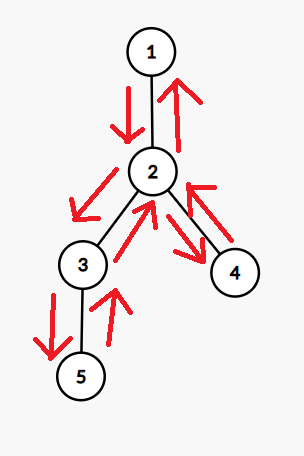
\includegraphics[width=0.3\textwidth]{pic.png}
    \end{center}
\end{ProblemSampleWithNote}

\ProblemSample{0-02.in}{0-02.out}

\clearpage

\ProblemSubtaskTitle

本題共有 1 組子任務,條件限制如下所示。

\begin{ProblemSubtaskTable}
    \ProblemSubtask{100}{無額外限制}
\end{ProblemSubtaskTable}